La tabla \ref{tab:angulos} reúne los ocho pares de ángulos, que son datos simulados como se explicó en el desarrollo experimental, junto con sus senos. La última columna es el índice de refracción que resulta de cada par por separado, calculado como $n = \sin\theta_i / \sin\theta_t$.

\begin{center}
\begin{tabular}{ccccc}
\hline
$\theta_i$ & $\theta_t$ & $\sin\theta_i$ & $\sin\theta_t$ & $n$ \\
(grados) & (grados) & & & \\
\hline
10 & 7.0  & 0.1736 & 0.1219 & 1.425 \\
20 & 14.5 & 0.3420 & 0.2504 & 1.366 \\
30 & 21.0 & 0.5000 & 0.3584 & 1.395 \\
40 & 27.0 & 0.6428 & 0.4540 & 1.416 \\
50 & 33.0 & 0.7660 & 0.5446 & 1.407 \\
60 & 37.5 & 0.8660 & 0.6088 & 1.423 \\
70 & 42.5 & 0.9397 & 0.6756 & 1.391 \\
80 & 46.0 & 0.9848 & 0.7193 & 1.369 \\
\hline
\end{tabular}
\captionof{table}{Ángulos de incidencia y de refracción simulados, sus senos y el índice de refracción que da cada pareja.}
\label{tab:angulos}
\end{center}

Lo primero que salta a la vista es que el rayo siempre se acerca a la normal al entrar al acrílico. Ningún ángulo de refracción supera al de incidencia, justo lo que se espera al pasar a un medio donde la luz va más lenta.

Siguiendo la ecuación \eqref{eq:recta}, se graficó $\sin\theta_i$ contra $\sin\theta_t$ y se ajustó una recta que pasa por el origen. El resultado fue
\begin{equation}
\sin\theta_i = 1.396 \, \sin\theta_t ,
\label{eq:ajuste}
\end{equation}
con un coeficiente de determinación $R^2 = 0.9986$. La figura \ref{fig:grafica} muestra los datos y la recta.

\begin{center}
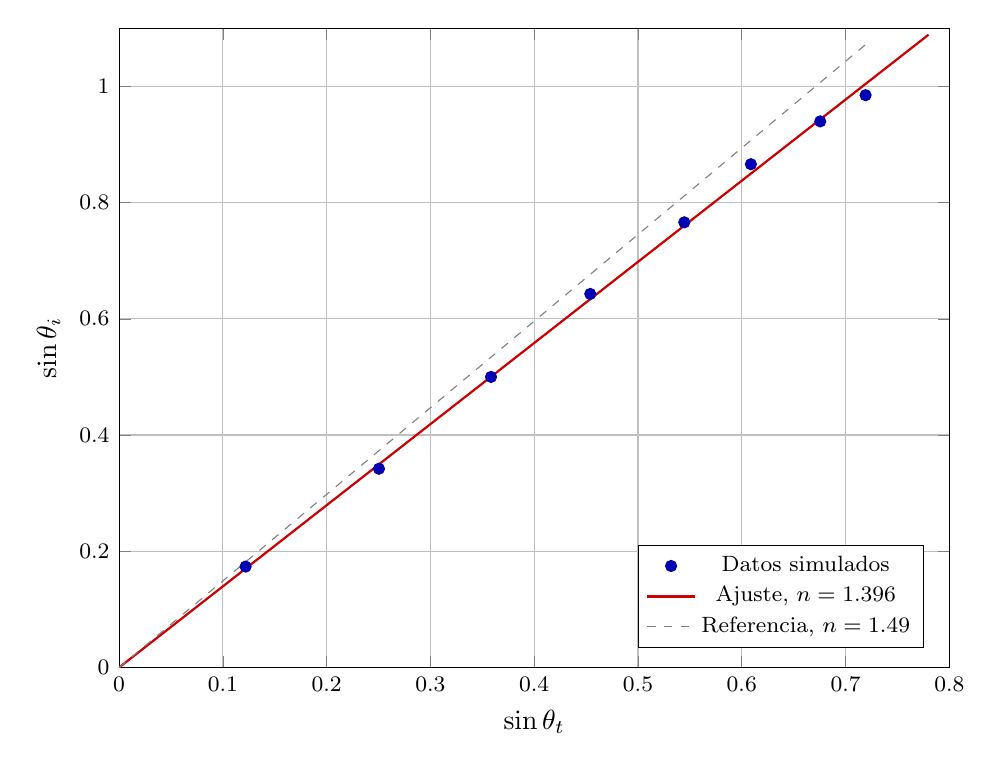
\begin{tikzpicture}
\begin{axis}[
    width=\columnwidth,
    height=0.8\columnwidth,
    xlabel={$\sin\theta_t$},
    ylabel={$\sin\theta_i$},
    xmin=0, xmax=0.8,
    ymin=0, ymax=1.1,
    grid=major,
    legend pos=south east,
    legend style={font=\footnotesize},
    tick label style={font=\footnotesize},
]
\addplot[only marks, mark=*, color=blue!70!black] coordinates {
    (0.1219,0.1736) (0.2504,0.3420) (0.3584,0.5000) (0.4540,0.6428)
    (0.5446,0.7660) (0.6088,0.8660) (0.6756,0.9397) (0.7193,0.9848)
};
\addlegendentry{Datos simulados}
\addplot[domain=0:0.78, samples=2, thick, color=red!80!black] {1.396*x};
\addlegendentry{Ajuste, $n = 1.396$}
\addplot[domain=0:0.72, samples=2, dashed, color=gray] {1.49*x};
\addlegendentry{Referencia, $n = 1.49$}
\end{axis}
\end{tikzpicture}
\captionof{figure}{Seno del ángulo de incidencia contra seno del ángulo de refracción. La recta roja es el ajuste de la ecuación \eqref{eq:ajuste} y la línea punteada es la que se obtendría con el índice de referencia del acrílico.}
\label{fig:grafica}
\end{center}

Si en lugar de la pendiente se promedian los ocho valores de la última columna de la tabla, se obtiene $n = 1.399 \pm 0.023$, prácticamente lo mismo.
